\documentclass[12pt,a4j,notitlepage]{jreport}
\usepackage[dvipdfmx]{graphicx}     %図を表示するのに必要
\usepackage[dvipdfmx]{color}        %jpgなどを表示するのに必要
\usepackage{amsmath,amssymb}        %数学記号を出すのに必要
\usepackage{setspace}
\usepackage{ascmac}
\usepackage{comment}
 \usepackage{url}
\usepackage{subfigure}
\usepackage{here}
%PDFの機能(しおり機能、ハイパーリンク機能)が使えるようにする
%しおりの文字化けを防ぐ

\usepackage{atbegshi}
\ifnum 42146=\euc"A4A2
\AtBeginShipoutFirst{\special{pdf:tounicode EUC-UCS2}}
\else
\AtBeginShipoutFirst{\special{pdf:tounicode 90ms-RKSJ-UCS2}}
\fi
%hyperrefのverが2007-06-14 6.76i以前の時は↓
%\AtBeginShipoutFirst{\special{pdf:tounicode 90ms-RKSJ-UCS2}}
%\usepackage[dvipdfmx,bookmarkstype=toc,colorlinks=true,urlcolor=blue,linkcolor=blue,
%citecolor=blue,linktocpage=true,bookmarks=true,setpagesize=false,
%pdftitle={論文のタイトルをここに入れる},
%pdfauthor={自分の名前(著作者)をここに入れる},%
%pdfsubject={Bachelor's thesis in 2013(2013年の学士論文という意味!)}]{hyperref}
\usepackage[numbers,sort]{natbib}
\usepackage{tocbibind}%目次、表一覧、図一覧をしおりに入れる

%式、図、表番号の付け方の再定義
\makeatletter
    \renewcommand{\theequation}{%
    \thesection.\arabic{equation}}
    \@addtoreset{equation}{section}
    \def\thefigure{\thesection.\arabic{figure}}
    \@addtoreset{figure}{section}
    \renewcommand{\thetable}{%
    \thesection.\arabic{table}}
    \@addtoreset{table}{section}
\makeatother

\renewcommand\bibname{参考文献}         %関連図書->参考文献
\newcommand{\figref}[1]{図~\ref{#1}} %図1等の定義

%大きなフォントの定義(表紙用)
\def\HUGE{\fontsize{36pt}{40pt}\selectfont} %\fontsize{フォントの大きさ}{baselineskip}


 \renewcommand{\baselinestretch}{1.5}


%ここから本文
\begin{document}
%題名
\begin{titlepage}
\begin{center}\begin{LARGE}
{\large 2019年度\hspace{3em}卒  業  研  究  論  文}\vspace{3em}\\


\textbf{\HUGE{多目的進化計算における}}\\
\textbf{\HUGE{トーナメント選択の有効性の評価}}\\
\vspace{14em}


\vspace{0.8em}
{\LARGE\bf }

{東京理科大学 工学部 経営工学科}\\\vspace{0.8em}
{ 4415010 \hspace{3em}井上 舜也}\\
\vspace{1em}
{ 指導教員:  藤井 孝藏教授,立川 智章講師}

\end{LARGE}\end{center}
\end{titlepage}

\pagenumbering{roman}   %目次のページはローマ数字
\tableofcontents




\chapter{序論}
\pagenumbering{arabic}  %本文についてはアラビア数字(この命令は必要)
\section{研究背景}
最適化とは, 与えられた制約条件下において何らかの評価指標の最適な条件を探索することである. 最適化は, 工学・産業・経済などの多くの分野で用いられている.一般に, 最適化とは一つの目的に対して最適化を行う単目的最適化を意味する.
しかし,実世界の最適化問題の多くは,複数の目的が存在する多目的最適化問題である.
そこで近年,トレードオフ関係にある複数の目的関数を同時に最適化する多目的最適化問題(Multi-objective Optimization Ploblems: MOP)に関する研究が盛んに行われている\cite{Li2009}.
複数の目的を同時に最適化すると全ての目的関数で最適値を選択する事は難しく,ある目的関数では最適値を取れなくなる場合が多い.そのような目的間の関係をトレードオフ関係と呼ぶ.
このトレードオフ関係にある多目的について最適化を行うとどの目的関数でも他の解に対して全て勝っている解が得られる.この解のことをパレート最適解と呼ぶ.パレート最適解は唯一に定まらず,集合として得ら れる.この集合のことをパレートフロントと呼ぶ.
パレート最適解を効率的に探索する手法の中でも,代表的な手法として遺伝的アルゴリズム(Genetic Algorithm :  GA)がある.これは生物の遺伝と進化を模倣した解探索手法であり,評価,選択,交叉,突然変異を繰り返し行うことで最適解を探索する手法である.多目的進化計算手法(Multi-Objective Evolutionary Algorithm : MOEA)はGAを多目的最適化に対応させた手法である.しかし,GAの過程で初期収束や解探索の停滞などの問題が起こることがある。これらの問題を解決するためには,解集団の多様性を限りなく保ち,親個体ペアからより優れた個体を作り出す必要がある.そのため,多くの手法で親個体ペアの選択にトーナメント選択が用いられているが,それが進化に及ぼす影響について十分調べられていない.

\section{先行研究}
先行研究では目的関数を3に絞り,多目的進化計算にNSGA-IIを用いて親個体選択手法の一つであるトーナメント選択に着目し,ベンチマーク問題を用いてトーナメント選択が進化に与える影響を調べることを目的とし,ランダム選択との比較を行った.その結果, NSGA-IIを用いた3目的の計算では,トーナメント選択が収束性に与える影響はあまり大きくないと考えられるということが分かった.しかし,これは評価指標がGDであり,収束性については述べられているが,大切な指標の一つである解の多様性に関しては考慮されてない.

また目的関数が3目的に関して調べられているが, NSGA-IIによる多目的最適化では,一般的に目的数が2か3の問題に対して良好に機能するが,さらに目的数が増加すると,最適化が困難になることが確認されている\cite{h.i}.

\section{研究目的}
本研究ではMOEAにおける親個体選択手法および次世代個体選択法の一つであるトーナメント選択に着目し,様々なベンチマーク問題を用いてトーナメント選択の進化に与える影響が目的関数によってどれだけ変わるかを調べることを目的とし,ランダム選択との比較を行う.その際の評価指標には後述するHyperVolumeを用いる.

本研究では目的関数は3,5,7に限定して行い,多目的進化計算にはNSGA-II,そして目的関数の増加に対応できるように改良されてつくられたNSGA-III,IBEAを用いて行う.

\section{本論文の構成}
1章では, 本論文における研究背景, 研究目的について述べた.

2章では, 多目的最適化に関する概念や, 計算手法, 親個体選択法であるトーナメント選択など本研究に関わる内容をまとめる.

3章では, ベンチマーク問題,評価指標,計算条件など実験結果を理解する上で必要になるであろう内容についてまとめる.

4章では, 3章で定めた計算条件の下で実験を行い,トーナメント選択が進化に与える影響について論じる.

5章では, 本研究の結論, 今後の課題について述べる.

\chapter{多目的最適化}
はじめに, 本章では多目的最適化に関して説明する.
2.1節では, まず多目的最適化について, また多目的最適化で重要な概念となるパレート最適解について説明する.
2.2節では, 多目的進化計算手法を幾つか説明する.
2.3節では, 本研究で用いられるトーナメント選択について説明する.


\section{最適化}
最適化(optimization)とは,何かしらの価値基準に対して最も適した解を求めることである.工学設計ではこのような価値基準として,コスト,性能,重量などの様々な問題に応じて各々基準が取られる.一般に, 最適化とは一つの目的に対して最適化を行う単目的最適化を意味し,次のように定式化される.
\begin{eqnarray}
(MP)         目的&:& f(x) → min\\
         制約&:&x    \in  X.
\end{eqnarray}
ここで$x$は設計変数,$f(x)$は目的関数と呼ぶ.しかし,問題によっては最大化を求められる場合もある.そのような場合は$-f(x)$を最小化すれば良い.

\subsection{多目的最適化問題}
しかしながら,世の中には複数の評価基準を同時に考慮すべき問題が数多く存在する.このような複数の評価基準を考慮して同時に最適化を行うことを多目的最適化と呼ぶ.しかし,実際には,同時に全ての目的の最適化を実現することは難しいことが多い.なぜなら,多目的最適化における複数の評価基準は互いに競合することが多く,そのような場合にはただ1つの最適解は存在しないからである.例えば,計算機の設計問題において,性能の最大化や製造コストの最小化,重量の最小化といった全ての目的の最適化を行うことは一般的に難しく,そのトレードオフの関係を考慮し,最適化を行う必要がある.

このように,場合によっては互いに矛盾する目的をそれぞれ可能な限り最適化するというところに,多目的最適化の本質が存在する.与えられた設計変数と制約条件において,複数の目的関数に対して最小化(最大化)する問題を多目的最適化問題と呼び,一般に次のように定式化される.
\begin{eqnarray}
(MOP)         目的&:& f(x):=(f_1(x),f_2(x),..............,f_n(x)) → min\\
         制約&:&x    \in  X.
\end{eqnarray}

\subsection{パレート最適解}
トレードオフ関係にある多目的について最適化を行うとどの目的関数でも他の解に対して全て勝っている解が得られる.この解のことをパレート最適解と呼ぶ.パレート解は唯一に定まらず,集合として得られる.この集合のことをパレートフロントと呼ぶ.パレート最適解は, 多目的最適化問題における解の優越関係により定義される.
多目的最適化問題における解の優越関係の定義を以下に示す.
ここでは, 全ての目的が最小化問題と仮定した場合のみ示す.
\begin{eqnarray}
        f_i(x) &\leq & f_i(y)    \hspace{10mm}  \forall i \in \{1,2,3,.....,N\} \\
        f_i(x) & < & f_i(y)       \hspace{10mm} \forall i \in \{1,2,3,.....,N\} \\
        x,y &=& (x_1,x_2,....,x_n)
\end{eqnarray}

式(2.1.5)では, $x$が$y$に優越するという.
式(2.1.6)では, $x$が$y$に強い意味で優越するという.
この場合, $x$は$y$よりも良い解であることを意味する.
ある解を対象として, 強い意味で優越する解が存在しない場合, その解を弱パレート最適解と呼び, 優越する解が存在しない場合, パレート最適解と呼ぶ.

\section{多目的進化計算手法}
多目的最適化問題では,各目的関数がトレードオフ関係にある場合,一つの最適解を求めることは難しい.
多目的最適化問題を解く場合,パレート最適解の集合が求められることが望ましい.そこで,多点探索である進化計算を用いてパレート最適解の集合を求める方法が提案されている.進化計算とは,自然界における生物の進化を模倣した計算法の総称である.進化計算は,多点探索を行うことができる確率的最適化計算であり,多目的最適化に有効な手法として,注目を集めている.その代表的な手法として遺伝的アルゴリズム(Genetic Algorithm : GA)がある.
多目的進化計算手法(Multi-Objective Evolutionary Algorithm : MOEA)はGAを多目的最適化に対応したアルゴリズムである.
GAは自然界における生物の進化をモデル化した最適化手法である.
GAのフローチャートを図 \ref{fig:GA}に示す.
\begin{figure}[htbp]
	\begin{center}
		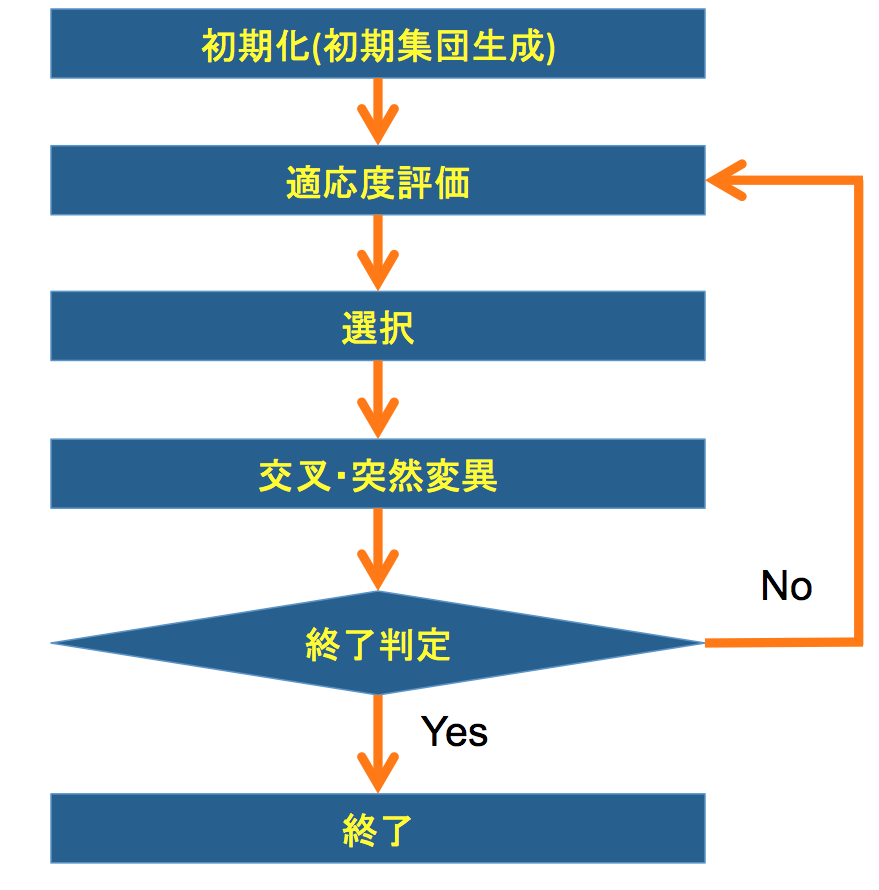
\includegraphics[width=0.8\linewidth]{img/GA.png}
             		\setlength{\abovecaptionskip}{0mm}
		\setlength{\belowcaptionskip}{0mm}
			\caption{GAのフローチャート}
	\label{fig:GA}
	\end{center}
\end{figure}

GAは, 初期化として決められた数の個体集合を生成する.
次に各個体の環境への適応度(目的関数の満足度)を計算し, 適応度の高い個体を次の世代に多く残す仕組みとなっている.
また, 適応度の高い個体に対して, 交叉及び突然変異を行うことで次世代におけるより良い解を生成する.
これらの操作の繰り返しによって最適な解を探索するのがGAの流れである.
またMOEAは一度に多数のパレート最適解を得ることができ, 勾配情報なども必要としないことから多目的最適化に効果的な手法と言われている.

本研究で用いる, MOEAの中でも有名な手法の3つについて説明する.
\subsection{Non-dominated Sorting Genetic Algorithms-II : NSGA-II}
NSGA-II\cite{Deb}はSrinvasらが提案したNon-dominated Sorting Genetic Algorithm(NSGA)に生存選択法としてエリート主義を導入したアルゴリズムであり, Debらによって提案された.
NSGA-IIは収束性の評価軸にパレートランキング法を, 多様性の評価軸として混雑距離を導入している.
パレートランキング法の概念図を図 \ref{fig:ranking}に示す.
\begin{figure}[htbp]
	\begin{center}
  \subfigure[Rank1の計算]{
		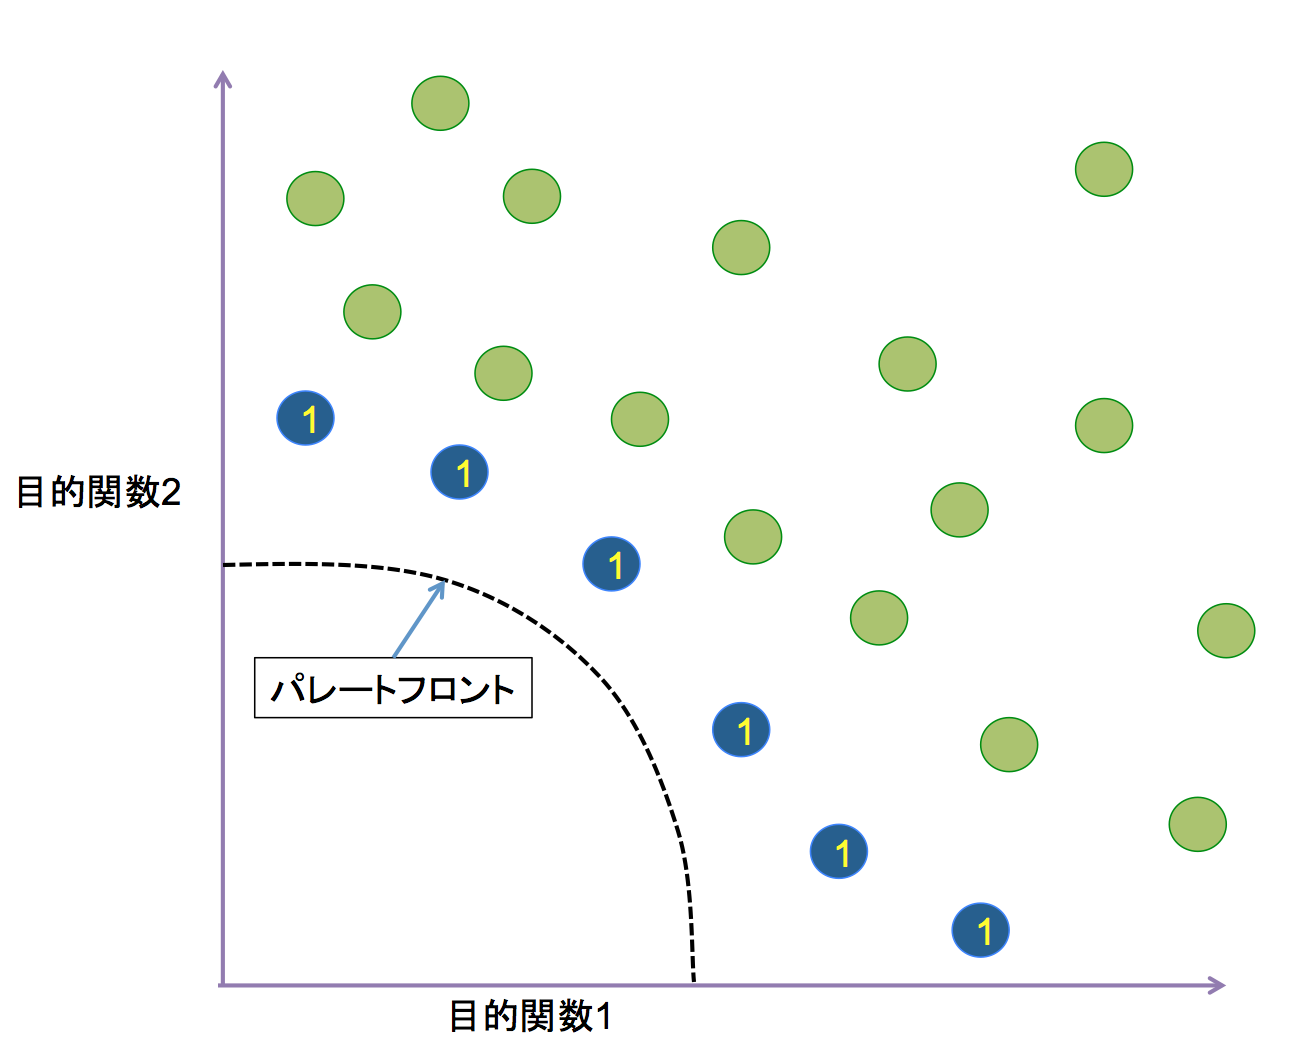
\includegraphics[width=0.3\linewidth]{img/Rank1.png}
		\label{fig:dtlz3_credit1}
		}
		 \subfigure[Rank2の計算]{
		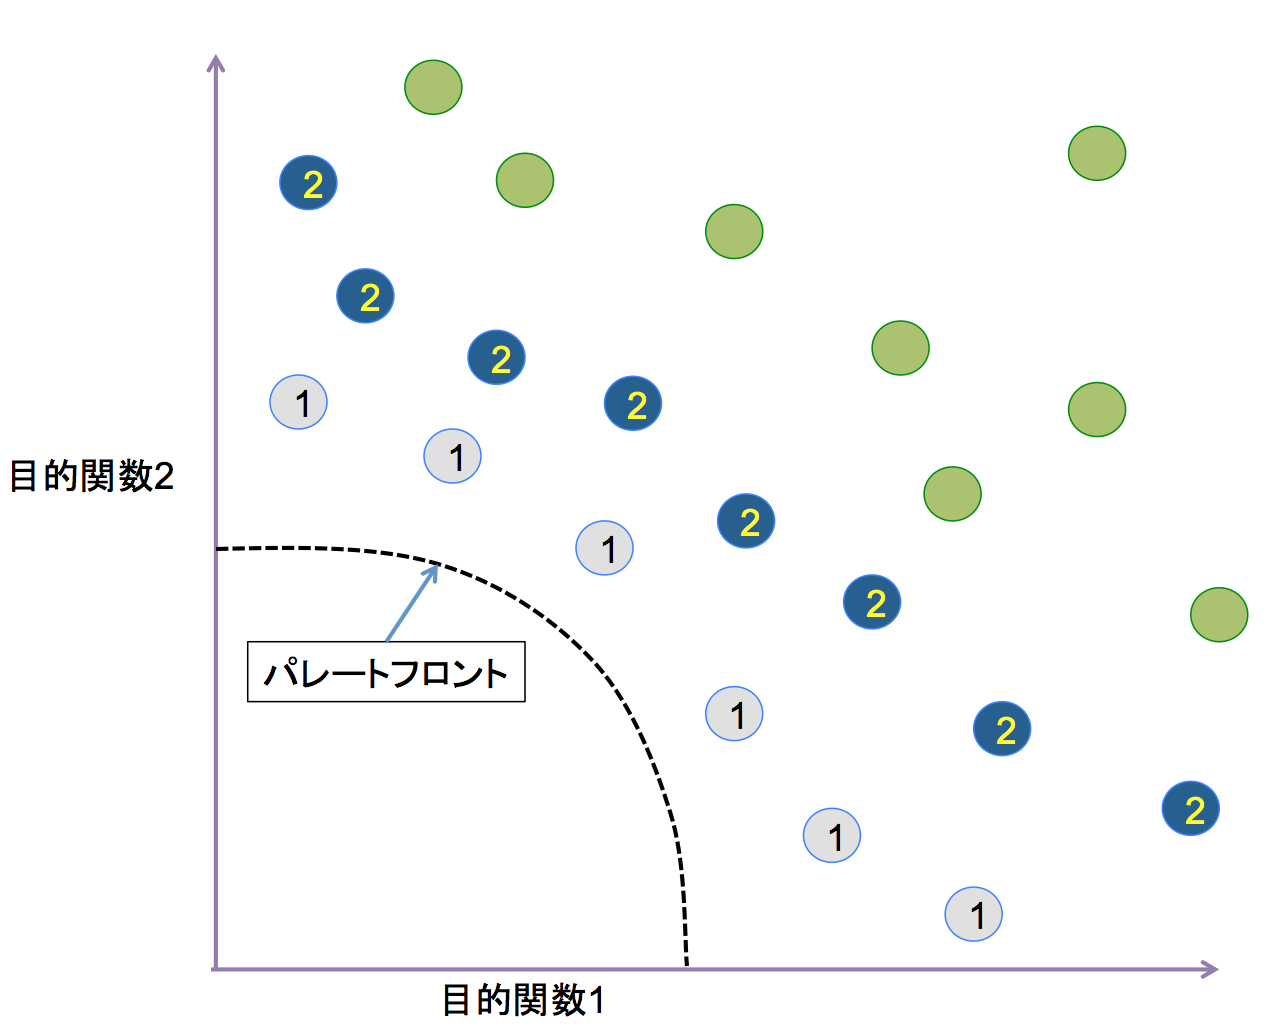
\includegraphics[width=0.3\linewidth]{img/Rank2.png}
		\label{fig:dtlz3_credit2}
		}
		\subfigure[Rank5の計算]{
		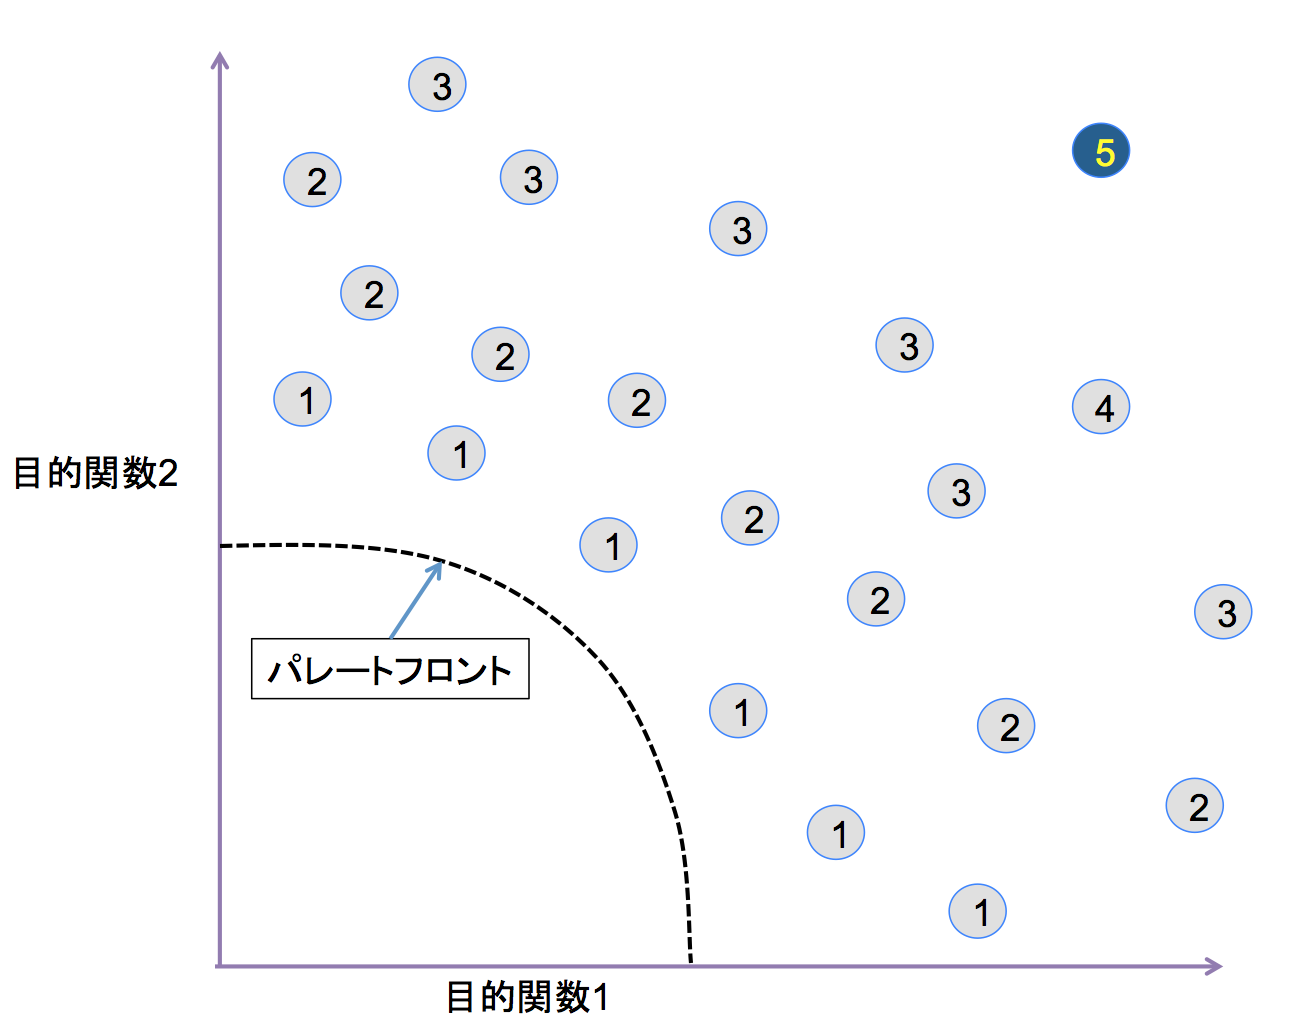
\includegraphics[width=0.3\linewidth]{img/Rank5.png}
		\label{fig:dtlz3_credit1_improve}
		}

             		\setlength{\abovecaptionskip}{0mm}
		\setlength{\belowcaptionskip}{0mm}
			\caption{パレートランキング法}
	\label{fig:ranking}
	\end{center}
\end{figure}
\vspace{3mm}
パレートランキング法では, 集合の中で他のどの個体にも支配されない解をRank1とする.
次に, Rank1の解を除いた集合の中で他のどの個体にも支配されない解をRank2とする.
この繰り返しを全個体でRankが決まるまで行う.
図\ref{fig:ranking}では, 最大Rankは5となる.
また, NSGA-IIではこのランキングの高速化した高速優越ソートを用いている.
高速優越ソートの手順を以下に示す.


\begin{enumerate}
\item 各個体に対して, 支配している個体の数と支配されている個体の数を同時に計算する.
\item Rank1の個体のみをリスト1にまとめる.
\item リストF$_1$に含まれる各個体が支配している個体に対して, 支配されている数を1ずつ引く.
\item 上記同様, Rank1(支配されている数が0)の個体のみをリストF$_2$にまとめる.
\item 1 $\sim$ 4を全個体が無くなるまで繰り返す.
\end{enumerate}

次に, 混雑距離について説明する.
混雑距離の概念図を図 \ref{fig:crowd}に示す.
\begin{figure}[htbp]
	\begin{center}
		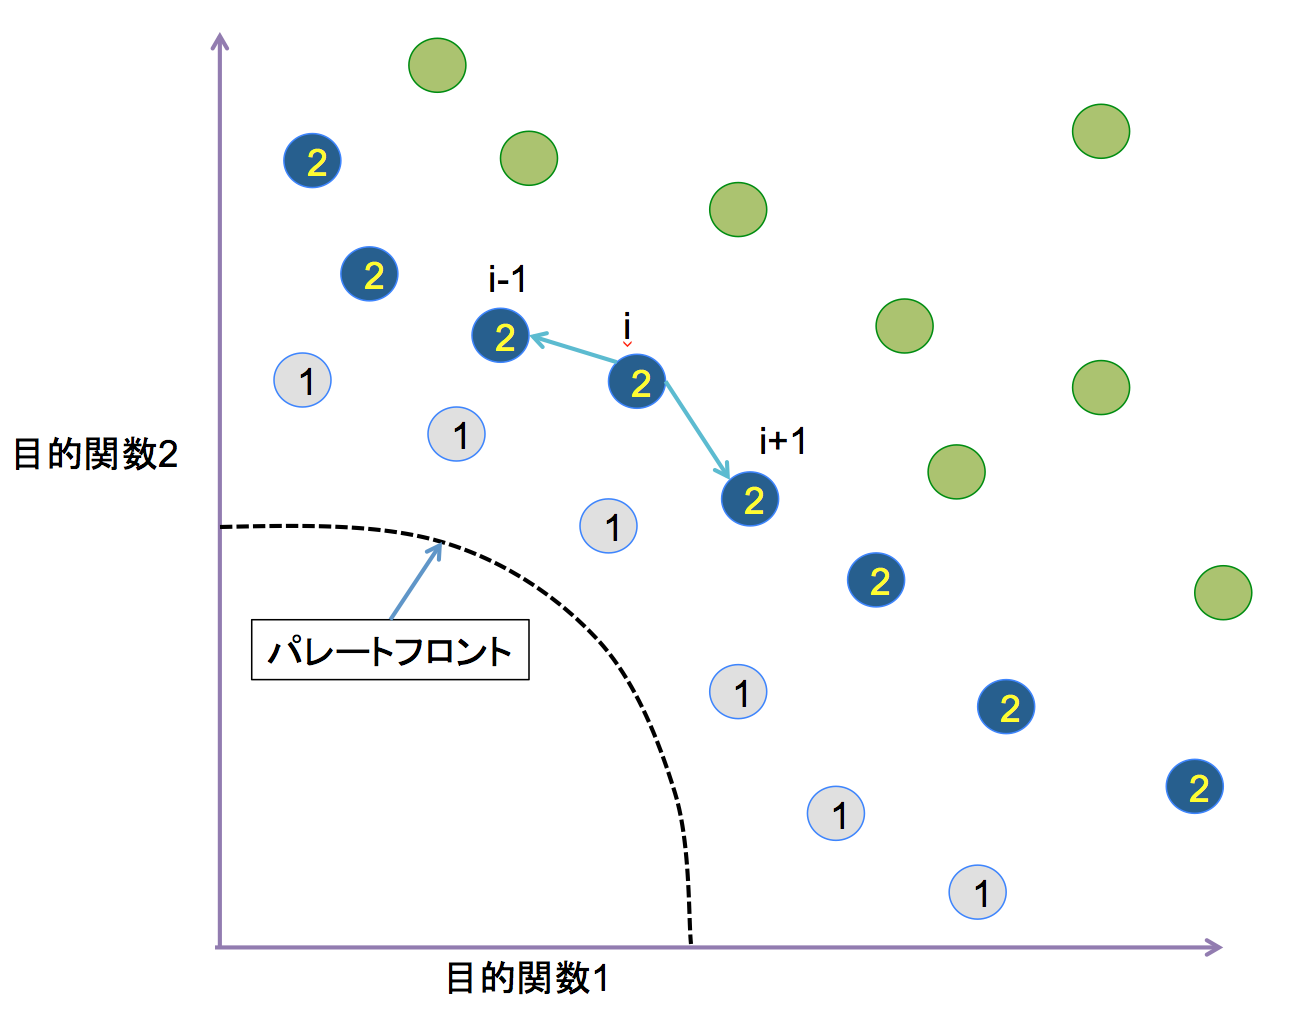
\includegraphics[width=0.7\linewidth]{img/Crowd.png}
             		\setlength{\abovecaptionskip}{0mm}
		\setlength{\belowcaptionskip}{0mm}
			\caption{混雑距離の計算法}
	\label{fig:crowd}
	\end{center}
\end{figure}

混雑距離は, 同一ランク内の集団を目的関数値でソートし, 両隣に隣接する個体との距離の和を計算する.
この計算は全個体で行われ, 各目的関数において端に位置する個体は無限大が割り振られる.

最後にNSGA-IIで用いられるエリート主義について説明する.
NSGA-IIのエリート主義の概念図を図 \ref{fig:nsgaii}に示す.
\begin{figure}[htbp]
	\begin{center}
		\includegraphics[width=0.7\linewidth]{img/NSGA-II.png}
             		\setlength{\abovecaptionskip}{0mm}
		\setlength{\belowcaptionskip}{0mm}
			\caption{NSGA-IIのエリート主義の概念図}
	\label{fig:nsgaii}
	\end{center}
\end{figure}

N個の個体で計算を行う場合, 毎世代N個の親個体P$_t$と, P$_t$から交叉, 突然変異によって新しく生成されるN個の子個体Q$_t$の合計2Nの個体が得られる.
2N個の個体から次の世代に使用するN個の親個体P$_{t+1}$の選択にエリート主義が使用される.
まずP$_t$とQ$_t$をマージした上で, パレートランキングによって各個体のランクを計算し, ランク順にソートを行う.
Rank1から順に, 合計数がNを超えないランクまでP$_{t+1}$に追加する.
P$_{t+1}$の個体数がNを超えてしまうランクでは, そのランク内の全個体で混雑距離を計算し, 値が大きい順にソートする.
そこで, P$_{t+1}$の個体数がNになるまで混雑距離のソートした順番に追加する.
端に位置する個体は混雑距離の値が無限大になるため, 必ず選択されるようになっている.

\subsection{Non-dominated Sorting Genetic Algorithms-III : NSGA-III}

NSGA-III\cite{Jain}は,Debらにより提案され,目的数が4以上の多目的最適化問題において,高い探索能力となるようNSGA-IIを改良した探索手法である.
NSGA-IIとの大きな違いは,多様性維持のための機構が異なっている点である.NSGA-IIIでは, reference lineに基づく個体選択により探索を行っている.

refenrence line および reference pointの概念を説明する.
初めに評価値空間上に均等に reference point を配置する. reference pointは,目的数を $M$ ,分割数を $p$ とすると
\[
  A = \left(
    \begin{array}{cc}
      M + p - 1 \\
            p
    \end{array}
  \right)
\]
個生成される. reference point の目的数が 3 ,分割数が 4 の例を\ref{fig:nsgaiii}に示す.
 \begin{figure}[htbp]
	\begin{center}
		\includegraphics[width=0.7\linewidth]{img/NSGA-III.png}
             		\setlength{\abovecaptionskip}{0mm}
		\setlength{\belowcaptionskip}{0mm}
			\caption{reference point の配置(M = 3 , p = 4)}
	\label{fig:nsgaiii}
	\end{center}
\end{figure}

reference lineとは,各 reference point と原点を通る線のことを表す.主な演算の流れはNSGA-IIと類似している.
NSGA-IIでは解の優越関係と混雑距離に基づいたエリート選択によって次世代個体の選択を行うが,
NSGA-IIIの次世代個体の選択では,次世代個体群の数が設定された個体数を超えない間は,NSGA-IIと同様に,ランクの高い個体から順に次世代個体に選択する.
探索個体数を超える場合には,混雑距離に代わり, reference line に基づいた選択により次世代に残す個体を決定する.以下に, reference line を用いた次世代個体の選択方法を説明する.

まず,個体 P$_i$ について,評価値空間上での距離が最も近い reference line L$_j$ を,個体 P$_i$に対する近傍ラインと定義する.また,L$_j$を近傍ラインとする個体を L$_j$に対する近傍個体と定義する.

\begin{enumerate}
\item すでに次世代個体に選択されている個体に対し,それぞれ近傍ラインを割り振る.
\item 近傍個体数の最も少ない reference line を選び,対象ランクの個体群のうち,その reference line の近傍個体の中から最も距離の近い個体を次世代個体群に加える.
\item 次世代個体群の数が設定された個体数を満たすまで 2 を繰り返す.
\end{enumerate}

reference line を用いることにより,目的関数の数が大きい最適化問題においても,高い収束性を有することが示されている.\cite{Jain}

\subsection{Indicator-Based Evolutionary Algorithm : IBEA}
IBEA\cite{Zitzler}は,Zitlerによって提案されたアルゴリズムである.これは, パレート優越関係とは別のメカニズによって個体の適応度の評価を行う手法である.
IBEAでは,Indicator functionとよばれる個体群全体を評価する関数を用い, Hypervolume\cite{Deb}が Indicator functionとして用いられることが多い.

Hypervolumeについて説明する.Hypervolume(HV)は任意の参照点$W$を用いて, 得られたパレート最適解集合の各点に対してhypercube $v_i$を生成し, $v_i$の和集合の領域が占める面積, 体積を計算する.
参照点は最適化方向とは反対方向に用意することが多く, 値が大きいほどその解集合が収束性と多様性に関して優れていることを意味する.

HVは次式で定式化される.
\begin{equation}
HV(S,W)=volume(\cup_{i=1}^{|S|} v_i) \label{eq:hv}
\end{equation}

ここで$S$は最適化によって得られたパレート最適解集合, $W$は参照点を示し, $v_i$は各hypercubeを示す.
HVの計算の概念図を図 \ref{fig:hvimg}に示す.
\begin{figure}[htbp]
	\begin{center}
		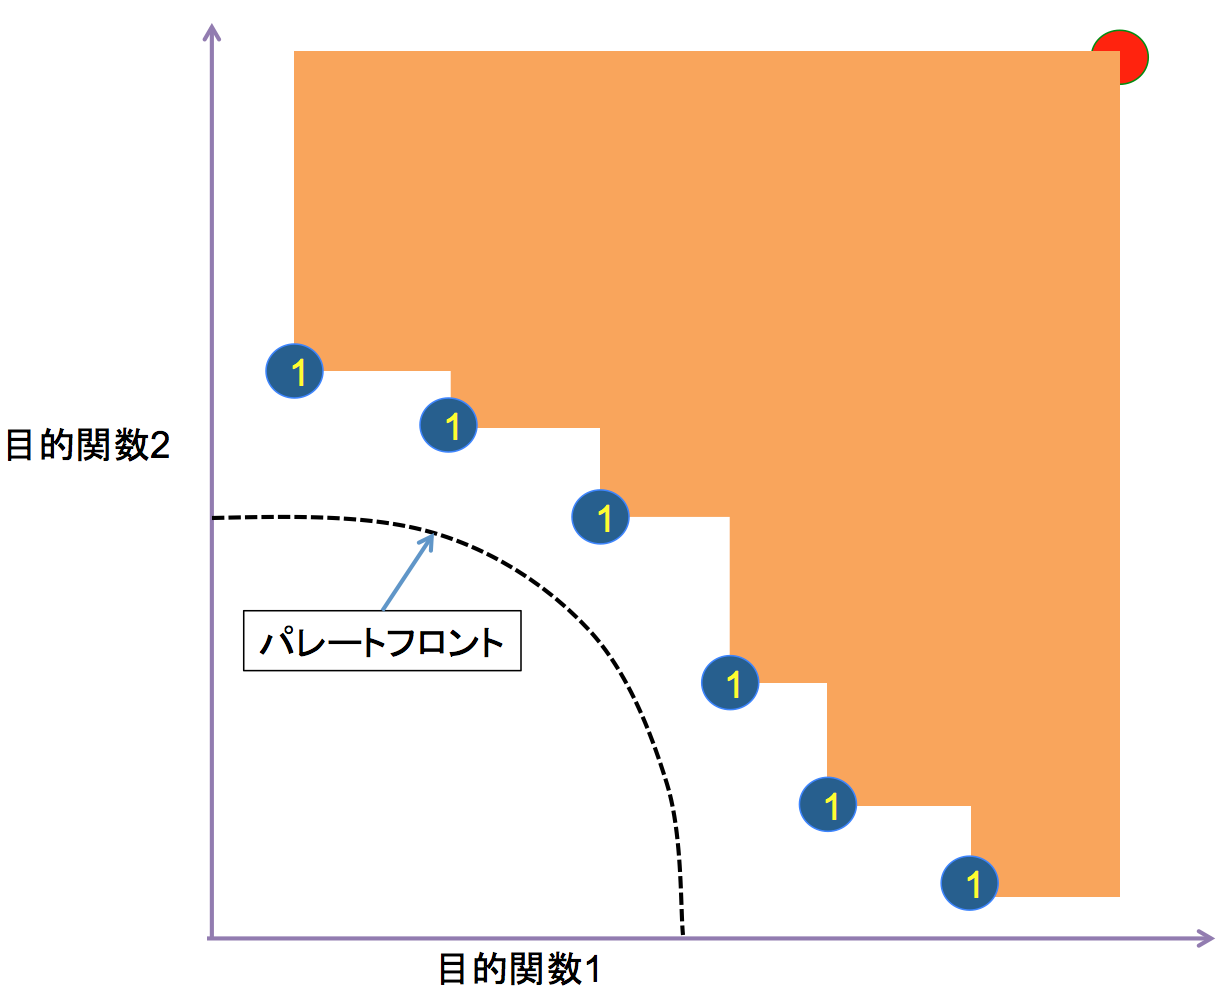
\includegraphics[width=0.7\linewidth]{img/HVimg.png}
             		\setlength{\abovecaptionskip}{0mm}
		\setlength{\belowcaptionskip}{0mm}
			\caption{HVの計算の概念図}
	\label{fig:hvimg}
	\end{center}
\end{figure}

図 \ref{fig:hvimg}は2目的における概念図であり, この場合総面積がHVの値となる.
HVでは, パレートフロントが既知ではない問題でも使用できるという強みがあるが, 目的数増加および個体数の増加に伴い,計算量が急激に増加し計算が困難になる.
IBEAは,個体群全体を評価するIndicator functionであるHypervolumeの最大化を行う単一目的最適化手法となる.

\section{トーナメント選択}
トーナメント選択は親個体選択手法の一つであり,多くの進化計算手法で用いられる.トーナメント選択は,設定された数の親個体候補が個体群からランダムに選択され,最も良い候を親個体とする.このとき親個体候補の数をトーナメントサイズと呼ぶ\cite{katai}.
図 \ref{fig:tournament}はトーナメントサイズが3のトーナメント選択の概念図である.
\begin{figure}[htbp]
	\begin{center}
		\includegraphics[width=0.7\linewidth]{img/tournament.png}
             		\setlength{\abovecaptionskip}{0mm}
		\setlength{\belowcaptionskip}{0mm}
			\caption{トーナメント選択の概念図(トーナメントサイズ:3)}
	\label{fig:tournament}
	\end{center}
\end{figure}


またトーナメント選択の影響を調べるために,ランダム選択との比較を行う.ランダム選択では,個体群から一個体をランダムに取り出し,親個体として選択する.ランダム選択はトーナメントサイズが1のトーナメント選択と同じ手法である.


\chapter{実験内容}
\section{多目的テスト問題}
多目的最適化問題では, 最終的に求めたいゴールはパレートフロントを形成することであり, その正確性が求められる.
しかし, 多くの多目的最適化問題はどこにパレートフロントが形成されるのかを知ることは困難であり, MOEAによって得られたパレートフロントが必ずしも正確なものとは限らない.
しかし, MOEAを開発する上でどれだけ正確なパレートフロントを形成出来るか知ることは非常に重要なことである.
そこで, 理論上のパレートフロントを既知なものとして開発されたのが多目的テスト問題である.

本研究では, 多目的テスト問題の中でも, DTLZシリーズ\cite{DTLZ}, WFGシリーズ\cite{WFG1,WFG2}の一部を用いる.

\subsection{DTLZテスト問題}
DTLZシリーズのテスト問題はDebらによって開発された目的数が可変なテスト問題である.
本研究では,その中からDTLZ 2,3,4を用いる.
DTLZ 2,3,4は2目的の場合, 図 \ref{fig:pareto_dtlz}に示すようなパレートフロントを持つ.
\begin{figure}[htbp]
	\begin{center}
		\includegraphics[width=0.7\linewidth]{img/DTLZ.png}
             		\setlength{\abovecaptionskip}{0mm}
		\setlength{\belowcaptionskip}{0mm}
			\caption{2目的におけるDTLZ 2,3,4のパレートフロント}
	\label{fig:pareto_dtlz}
	\end{center}
\end{figure}
DTLZ 2,3,4は2目的の場合, 原点を中心とした, 半径1の四半円周上にパレートフロントを形成する.
3目的になると, 同様に四半球面上にパレートフロントを形成するベンチーマーク問題である.

\subsection{WFGテスト問題}
WFGシリーズのテスト問題はHusbandらによって開発された目的数が可変であり, 一つの形式に従った上で問題に複雑性を追加していくテスト問題である.
WFGシリーズの各問題は形状関数, 変換関数という関数を用いてパレートフロンとの形状を決定している.
それぞれ異なる変換を行うため, 各問題のパレートフロントの形状は異なる.
本研究ではその中からWFG 1,2,6,8,9を用いる.

\section{評価指標}
多目的最適化によって得られたパレート最適解集合は複数の目的関数を持つことから目的関数値で優劣を評価することが出来ず, 収束性, 多様性という概念で評価される.
収束性は最適化方向(全目的で最小化問題なら原点方向)にどれだけパレート最適解集合が近づいているかということであり, 多様性は大まかに言えばどれだけ幅広い解集合となっているかということである.
一般的に, 得られた際に望ましいパレート最適解集合は目的空間においてより広がっており, 均一に分布しており, 密度の高いものが求められる.
本研究では,代表的な評価指標の一つであり,収束性と多様性を同時評価指標できるHypervolume(HV)を用いる.

\section{計算条件}
トーナメント選択とランダム選択との比較を行う際の計算条件を\ref{tb:keisan}に示す.
本研究では,目的数が可変であるベンチマーク問題のDTLZ,WFG問題の一部を扱う.
トーナメント選択を行う際のトーナメントサイズは本研究では2とする.

またHypervolumeの参照点として使用したものを表 \ref{tb:hvpoint}に示す.
\vspace{-2mm}
\begin{table}[h]
\begin{center}
\begin{tabular}{cc}
\begin{minipage}{1\hsize}
\begin{center}
\caption{計算条件}
\label{tb:keisan}
\begin{tabular}{|c|c|}
\hline
テスト問題&DTLZ2,3,4 WFG1,2,6,8,9 \\
\hline
進化計算手法&NSGA-II,NSGA-III,IBEA\\
\hline
親個体選択手法&ランダム選択,トーナメント選択\\
\hline
交叉手法&SBX\\
\hline
突然変異手法&polynomical mutatation\\
\hline
目的数&3,5,7\\
\hline
設計変数&12\\
\hline
集団サイズ&100\\
\hline
世代数&100\\
\hline
試行回数&10\\
\hline
\end{tabular}
\end{center}
\end{minipage}
\end{tabular}
\end{center}
\end{table}


\vspace{+2mm}
\begin{table}[h]
\begin{center}
\begin{tabular}{cc}
\begin{minipage}{1\hsize}
\begin{center}
\caption{Hypervolumeの参照点}
\label{tb:hvpoint}
\begin{tabular}{|c||c|c|c|}
\hline
テスト問題&3目的&5目的&7目的 \\
\hline
DTLZ2,4&(1.5,1.5,1.5)&(1.5,1.5,1.5,1.5,1.5)&(1.5,1.5,1.5,1.5,1.5,1.5,1.5)\\
\hline
DTLZ3&(225,225,225)&(225,225,225,225,225)&(225,225,225,225,225,225,225)\\
\hline
WFG1,2,6,8,9&(3.0,6.0,9.0)&(3.0,6.0,9.0,12.0,15.0)&(3.0,6.0,9.0,12.0,15.0,18.0,21.0)\\
\hline
\end{tabular}
\end{center}
\end{minipage}
\end{tabular}
\end{center}
\end{table}

\chapter{結果と考察}
表3.2.1および3.2.2の条件で実験を行う.

本研究では目的関数による値の変化をたどるため,全10試行の評価指標値から,平均値を計算し,参照点の座標でわった結果をを図4.1.1〜4.2.5に示す.これらの図は,横軸が目的関数の数,縦軸がHVの値を示した図となっている.

\section*{DTLZ問題}
図4.0..1〜4.0.3はそれぞれDTLZ問題での結果である.

図4.0.1および図4.0.2からDTLZ2,3ではどの進化計算手法においても目的関数の数によらず,トーナメントとランダムによる値の差が非常に小さいことが確認できる.

また図4.0.3からDTLZ4では3目的の場合に,NSGA-IIおよびNSGA-IIIではトーナメント選択が優位,IBEAではランダム選択が優位になっているが,目的関数の増加によりその差は非常に小さなものとなる.

よって,DTLZ問題では目的関数の数が大きい場合に,トーナメント選択の影響は非常に小さいものになることが確認できる.

\vspace{+2mm}
\section*{WFG問題}
図4.0.4〜4.0.8はそれぞれWFG問題での結果である.

図4.0.4〜4.0.7ではNSGA-IIにおいて差があらわれやすくなっているが,その差は小さいことが確認できる

また図4.0.8ではIBEAにおいて差があらわれやすくなっているが,この差も小さいことが確認できる.

よって,WFG問題では目的関数の数によらず,トーナメント選択の影響は小さいものになることが確認できる.

\section*{考察}
結果として,多くのベンチマーク問題では目的関数の数が大きい場合に,トーナメント選択の影響は非常に小さいものになることが確認できる.
これは,目的関数の数が大きくなることによって,パレート最適解の数が増え,進化計算の初期段階で個体間の適応度の差が小さくなり,選択圧がかかりにくくなるからではないかと考えられる.

また,本研究で用いたDTLZ問題において,どの進化計算手法においてもトーナメント選択とランダム選択のグラフが非常に似た形であらわれたのにはパレートフロントの形状が同一であることが関係しているのではないかと考えられる.

\vspace{+2mm}
\begin{figure}[H]
\begin{center}
   				\subfigure[NSGA-II]{
				\includegraphics[width=0.5\linewidth]{NSGA-II/img/DTLZ2.png}

				}
				\subfigure[NSGA-III]{
				\includegraphics[width=0.5\linewidth]{NSGA-III/img/DTLZ2.png}

				}
				\subfigure[IBEA]{
				\includegraphics[width=0.5\linewidth]{IBEA/img/DTLZ2.png}

				}
				\end{center}
				\setlength{\abovecaptionskip}{0mm}
\setlength{\belowcaptionskip}{0mm}
\vspace{-2mm}
			\caption{DTLZ2の比較}

	\end{figure}
\vspace{+2mm}
\begin{figure}[H]
\begin{center}
   				\subfigure[NSGA-II]{
				\includegraphics[width=0.5\linewidth]{NSGA-II/img/DTLZ3.png}

				}
				\subfigure[NSGA-III]{
				\includegraphics[width=0.50\linewidth]{NSGA-III/img/DTLZ3.png}

				}
				\subfigure[IBEA]{
				\includegraphics[width=0.50\linewidth]{IBEA/img/DTLZ3.png}

				}
				\end{center}
				\setlength{\abovecaptionskip}{0mm}
\setlength{\belowcaptionskip}{0mm}
\vspace{-2mm}
			\caption{DTLZ3の比較}

	\end{figure}
\vspace{+2mm}
\begin{figure}[H]
\begin{center}
   				\subfigure[NSGA-II]{
				\includegraphics[width=0.5\linewidth]{NSGA-II/img/DTLZ4.png}

				}
				\subfigure[NSGA-III]{
				\includegraphics[width=0.5\linewidth]{NSGA-III/img/DTLZ4.png}

				}
				\subfigure[IBEA]{
				\includegraphics[width=0.5\linewidth]{IBEA/img/DTLZ4.png}

				}

				\end{center}

				\setlength{\abovecaptionskip}{0mm}
\setlength{\belowcaptionskip}{0mm}
\vspace{-2mm}
			\caption{DTLZ4の比較}

	\end{figure}



\vspace{+2mm}
\begin{figure}[H]
\begin{center}
   				\subfigure[NSGA-II]{
				\includegraphics[width=0.5\linewidth]{NSGA-II/img/WFG1.png}

				}
				\subfigure[NSGA-III]{
				\includegraphics[width=0.5\linewidth]{NSGA-III/img/WFG1.png}

				}
				\subfigure[IBEA]{
				\includegraphics[width=0.5\linewidth]{IBEA/img/WFG1.png}

				}
				\end{center}
				\setlength{\abovecaptionskip}{0mm}
\setlength{\belowcaptionskip}{0mm}
\vspace{-2mm}
			\caption{WFG1の比較}

	\end{figure}
\vspace{+2mm}
\begin{figure}[H]
\begin{center}
   				\subfigure[NSGA-II]{
				\includegraphics[width=0.5\linewidth]{NSGA-II/img/WFG2.png}

				}
				\subfigure[NSGA-III]{
				\includegraphics[width=0.5\linewidth]{NSGA-III/img/WFG2.png}

				}
				\subfigure[IBEA]{
				\includegraphics[width=0.5\linewidth]{IBEA/img/WFG2.png}

				}
				\end{center}
				\setlength{\abovecaptionskip}{0mm}
\setlength{\belowcaptionskip}{0mm}
\vspace{-2mm}
			\caption{WFG2の比較}

	\end{figure}
\vspace{+2mm}
\begin{figure}[H]
\begin{center}
   				\subfigure[NSGA-II]{
				\includegraphics[width=0.5\linewidth]{NSGA-II/img/WFG6.png}

				}
				\subfigure[NSGA-III]{
				\includegraphics[width=0.5\linewidth]{NSGA-III/img/WFG6.png}

				}
				\subfigure[IBEA]{
				\includegraphics[width=0.5\linewidth]{IBEA/img/WFG6.png}

				}
				\end{center}
				\setlength{\abovecaptionskip}{0mm}
\setlength{\belowcaptionskip}{0mm}
\vspace{-2mm}
			\caption{WFG6の比較}

	\end{figure}
\vspace{+2mm}
\begin{figure}[H]
\begin{center}
   				\subfigure[NSGA-II]{
				\includegraphics[width=0.5\linewidth]{NSGA-II/img/WFG8.png}

				}
				\subfigure[NSGA-III]{
				\includegraphics[width=0.5\linewidth]{NSGA-III/img/WFG8.png}

				}
				\subfigure[IBEA]{
				\includegraphics[width=0.5\linewidth]{IBEA/img/WFG8.png}

				}
				\end{center}
				\setlength{\abovecaptionskip}{0mm}
\setlength{\belowcaptionskip}{0mm}
\vspace{-2mm}
			\caption{WFG8の比較}

	\end{figure}
\vspace{+2mm}
\begin{figure}[H]
\begin{center}
   				\subfigure[NSGA-II]{
				\includegraphics[width=0.5\linewidth]{NSGA-II/img/WFG9.png}

				}
				\subfigure[NSGA-III]{
				\includegraphics[width=0.5\linewidth]{NSGA-III/img/WFG9.png}

				}
				\subfigure[IBEA]{
				\includegraphics[width=0.5\linewidth]{IBEA/img/WFG9.png}

				}
				\end{center}
				\setlength{\abovecaptionskip}{0mm}
\setlength{\belowcaptionskip}{0mm}
\vspace{-2mm}
			\caption{WFG9の比較}

	\end{figure}



\chapter{まとめ}
\section{結論}
本論文では,多目的進化計算におけるトーナメント選択の有効性が目的関数の数によって如何に変化するか確認を行った.そのために,3種類の代表的な多目的進化計算手法と8種類のベンチマーク問題を用いることでトーナメント選択の有効性を検証をした.

その結果,本実験で用いたベンチーマーク問題においては,目的関数の数が小さい場合に,トーナメント選択が多少有効である場合があるが,目的関数の数が大きい時はトーナメント選択の影響が非常に小さいことが確認できた.

\section{今後の課題}
今後の課題として,集団サイズが多ければその分多様性は増すことが考えられるので集団サイズを増やしての検証が必要である.

また集団サイズによる変化がない場合にはトーナメント選択以外の親個体選択法の提案が必要である.

そして,本実験で親個体選択が進化に与える影響が非常に小さい可能性が浮かびあがったため,突然変異など他の手法に注目する必要性がある.

\begin{thebibliography}{99}
  \bibitem{Li2009} H.Li and Q. Zhang, Multiobjective optimization problems with complicated pareto sets, moea/d and nsga-ii,$Evolutionary Computation, IEEE Transactions$..., 2009.
   \bibitem{h.i}  H. Ishibuchi, N. Tsukamoto and Y. Nojima, “Evolutionary many-objective optimization: A short review,” In Proceedings of 2008 IEEE Congress on Evolutionary Computation (CEC 2008),pp.2424-2431 2008.
   \bibitem{katai} 片井修,玄光男,大野勝久,石渕久生,河上,浩司,辻村泰寛,半田久志,林林,岡本東. 進化技術 第I巻基礎編,2010
  \bibitem{Deb} K. Deb, A. Pratap, S. Agarwal, and T. Meyarivan. A fast and elitist multiobjective genetic algorithm: NSGA-II,Evolutionary Computation,IEEE Transactions Vol.6,No.2, pp.182-197,2002
  \bibitem{Srinivas}N.Srinivas and K.Deb.Multiobjective optimization using nondominated sorting in genetic algorithms.Evolutionary Computation,Vol.2, No. 3, pp.221-248 1994
  \bibitem{Jain} Deb, K. and Jain, H.: An evolutionary many objective optimization algorithm using reference-point based non-dominated sort- ing approach, part I: Solving problems with box constraints, IEEE Transactions on Evolutionary Computation (TEVC),Vol.18,No.4,pp.577-601 2014
  \bibitem{Zitzler}E. Zitzler and S. Kunzil: Indicator-based selection in multiobjective search; Lecture Notes in Computer Science 3242: Parallel Problem Solving from Nature PPSN Vol.3, pp.832-842, Springer 2004
 \bibitem{DTLZ}
 K. Deb, L. Thiele, M. Laumanns, and E. Zitzler. Scalable multiobjective optimization test problems. In Proc. Congress Evolutionary Computation CEC'02,Vol.1,pp.825-830,May 2002.
\bibitem{WFG1}S. Huband, P. Hingston, L. Barone, and R. L. While. A review of multiobjective test problems and a scalable test problem toolkit. IEEE Trans. Evolutionary Computation,Vol.10,No.5,pp.477-506,2006.
\bibitem{WFG2}S. Huband, L. Barone, L. While, and P. Hingston. A scalable multiobjective test problem toolkit.Springer,2005


   \end{thebibliography}


\chapter*{謝辞}
本論文を作成するに当たって, 長期にわたり研究や論文執筆に際して様々なご指導を頂きました工学部情報工学科立川智章講師には心より御礼申し上げます.
立川講師には,最適化や進化計算の基礎に始まり,進化計算の応用事例やプログラミングの見方に至るまで,懇切丁寧にご指導いただき,数多くのアドバイスを頂きました.また,無知であった筆者にも寛大にご対応頂きましたことをこの場を借りて感謝申し上げます.
工学部情報工学科藤井孝藏教授および招聘研究員である浅田健吾様,関本諭志様,にも大変お世話になりました.
工学部経営工学専攻小川拓人氏には,プログラミング等でつまずいたときに大きなお力添えをしていただき,また資料の作成や発表の方法について多くのご指導を頂き,心より御礼申し上げます.
日々切磋琢磨し,辛いときには支え合い多くの時間を共に過ごした同期の皆様に感謝いたします.
秘書の幸野早苗様には,研究室での生活の多くをサポートして頂き,心地よい研究室生活を送ることができました.深く御礼申し上げます.
最後に, 東京理科大学での4年間, 勉学, 研究を行う機会を頂いた両親をはじめ, 本論文に携わって頂いた皆様に感謝の意を表し, 「多目的進化計算におけるトーナメント選択の有効性の評価」を締め括りたいと思います.


\end{document}
